%2024.May

\documentclass[12pt]{article}

\setlength{\topmargin}{-1.5cm}
\setlength{\textheight}{25cm}
\setlength{\textwidth}{17cm}
\setlength{\evensidemargin}{-0.25cm}
\setlength{\oddsidemargin}{-0.25cm}

%   \oddsidemargin  -0.10cm
%   \evensidemargin -0.10cm
%   \topmargin      -1.72cm
%   \textheight      24.5cm
%   \textwidth       16.0cm

%\pagestyle{empty}
%%%%%%%%%%%%%%%%%%%%%%%%
\usepackage{amssymb,amsmath,amsfonts}
\usepackage{amssymb,graphicx}
\usepackage{abstract}
%\date{}%, ${}^\dagger${FUJI Film Inc.}}}
% macro definition
\newcommand*{\Rset}{\mathbb{R}}
\newcommand*{\Zset}{\mathbb{Z}}
%----#<^_NSEDR_^#<ؖ#<^_NSEDR_^#<̏I���
\def\qed{{\ \vbox{\hrule\hbox{%
   \vrule height1.3ex\hskip0.8ex\vrule}\hrule
  }}\par}
\def\e{ \,{\rm e}}
%----vector variables
\def\bfvec#1{\mbox{\boldmath$#1$}}

\newtheorem{Definition}{Definition}
\newtheorem{Lemma}{Lemma}
\newtheorem{AuxiliaryProposition}{Auxiliary Proposition}
\newtheorem{Proposition}{Proposition}
\newtheorem{Theorem}{Theorem}
\newtheorem{Corollary}{Corollary}
\newtheorem{Remark}{Remark}
\newtheorem{Assumption}{Assumption}
\newfont{\stt}{cmtt8}
%%%%%%%%%%%%%%%%%%%%%%%%%
%%%%%%%%%%%%%%%%%%%%%%%%%

\begin{document}

\title{About an approximate formula for scattering amplitude by a disc}
\author{Fumihiro Chiba\thanks{https://github.com/chibaf}}
%------------------------
\maketitle

\begin{abstract}
A fundamental solution method gives an analytic representation of the approximate solution for the wave problem in the exterior region of a disc. The asymptotic behavior of this representation yields an approximate formula for the scattering amplitude.
\end{abstract}

\section{An approximate solution for reduced wave problem by FSM}
Consider the following reduced wave problem in the exterior domain of a disc with Dirichlet boundary condition. Let $a$ be the radius of a disc, and $k$ a wave number. Then the problem is represented as follows.
\begin{eqnarray*}
\left\{
\begin{array}{r}
\displaystyle -\Delta u -k^2 u = 0 \quad {\rm in} \; \Omega_e,\\
\displaystyle u=f \quad {\rm on} \; \Gamma_a, \\
\displaystyle \lim_{r \rightarrow \infty} \sqrt{r} \left\{\frac{\partial u}{\partial r}- \mathrm{i} k u \right\}=0,
\end{array}
\right.
\end{eqnarray*}
where
\begin{eqnarray*}
{\small \Omega_e=\{\bfvec{r}\in\Rset^2;\;|\bfvec{r}|>a\}, \; \Gamma_a=\{\bfvec{a}\in\Rset^2;\; |\bfvec{a}|=a\},}
\end{eqnarray*}
and $|\cdot|$ is the Euclidean norm in $\Rset^2$.


A positive number $\rho$ is the radius of a disc containing all source points. Let $N$ be a fixed positive integer. Then we define a basis function $G_j(\bfvec{r})$ through
\begin{displaymath}
G_j({\bfvec{r}}) = H_0^{(1)}(k|r\e^{\mathrm{i}\theta}- \rho \e^{\mathrm{i}{\theta}_j}|),
\quad \theta_j=j\frac{2\pi}{N},\quad 0 \leq j \leq N-1,
\end{displaymath}
where $H_0^{(1)}(\cdot)$ is the zeroth order Hankel function of the first kind, and the points $(r,\theta)$ and $(\rho,\theta_j)$ correspond to the complex numbers $r\e^{\mathrm{i}\theta}$ and $\rho \e^{\mathrm{i}{\theta}_j}$, respectively.

An approximate solution of the problem above is given as follows\cite{ushijima-chiba 1}.
\begin{displaymath}
u^{(N)}(\bfvec{r})=\sum^{N-1}_{j=0} Q_j G_j(\bfvec{r}),
\end{displaymath}
where $Q_j$ is the intensity of sources, and $\bfvec{r}$ corresponds to the polar coordinate $(r,\theta)$.

The intensity of sources $Q_j$ is computed as follows.
Introduce the following normalized parameters:
\begin{displaymath}
\gamma = \frac{\rho}{a}, \quad 
\delta = \frac{r}{a}, \quad 
\kappa = ka.
\end{displaymath}
Then the basis function is represented as follows.
\begin{displaymath}
G_j({\bfvec{r}}) = H_0^{(1)}(\kappa|\delta- \gamma \e^{-\mathrm{i}(\theta -{\theta}_j)}|),
\quad 0 \leq j \leq N-1.
%\label{basis function 2}
\nonumber
\end{displaymath}
Introduce the kernel function:
\begin{displaymath}
g(\theta)=H^{(1)}_0(\kappa|1-\gamma \e^{-i\theta}|).
\end{displaymath}
The intensity of sources $Q_j$ is given as follows.
\begin{displaymath}
Q_j=\frac{1}{N}\sum^{N-1}_{k=0}\frac{F^{(N)}_k}{G^{(N)}_k}\e^{\mathrm{i}j\theta_k} \quad {\rm for}\;0 \le j\ \le N-1,
\end{displaymath}
where
\begin{displaymath}
F^{(N)}_k = \frac{1}{N}\sum^{N-1}_{j=0}f(\bfvec{a}_j)\e^{-\mathrm{i}k\theta_j}, \quad G^{(N)}_n = \frac{1}{N}\sum^{N-1}_{j=0}g(\theta_j)\e^{-\mathrm{i}n\theta_j},
\end{displaymath}
where $\bfvec{a}_j$ corresponds to the polar coordinate $(a,\theta_j)$.


\section{An approximate formula for scattering amplitude}
An approximate scattering amplitude $A^{(N)}(\theta)$ for the above problem is given as follows\cite{chiba-ushijima 1},\cite{chiba-ushijima 2}.
\begin{eqnarray*}
A^{(N)}(\theta)=\lim_{r\rightarrow\infty}\left(\frac{\e^{\mathrm{i}r}}{\sqrt{r}}\right)^{-1}u^{(N)}(\bfvec{r})=\sum^{N-1}_{j=0} \sqrt{\frac{2}{\pi k}}\e^{-\frac{\mathrm{i}\pi}{4}}Q_j \e^{-\mathrm{i} \kappa \gamma \cos(\theta-\theta_j)} \\
\quad {\rm with}\;\theta_j=\frac{2\pi j}{N},
\label{A^(N)}
\end{eqnarray*}
where an asymptotic formula of Hankel functions\cite{Abramowitz-Stegun} is used.

Then an approximate far-field coefficient\cite{Bowman-Senior-Uslenghi} $P^{(N)}(\theta)$ is given as follows.
\begin{displaymath}
P^{(N)}(\theta)=\sqrt{\frac{\pi k}{2}}\e^{\mathrm{i}\frac{\pi}{4}} A^{(N)}(\theta).
\end{displaymath}

The scattering cross section $\sigma(\theta)$ is computed as follows\cite{Bowman-Senior-Uslenghi}.
\begin{displaymath}
\sigma(\theta)=\lim_{r\rightarrow\infty}2\pi r \left|\frac{u(\bfvec{r})}{u_i(\bfvec{r})}\right|^2,
\end{displaymath}
where $u_i(\bfvec{r})$ is an incident wave.

Suppose:
\begin{displaymath}
\lim_{r\rightarrow\infty}|u_i(\bfvec{r})|=1.
\end{displaymath}
The scattering wave $u(\bfvec{r})$ is expected to behave in the far-field as follows.
\begin{displaymath}
u(\bfvec{r}) \sim \frac{\e^{\mathrm{i}kr}}{\sqrt{r}}A(\theta) \quad {\rm as}\;r\rightarrow\infty,
\end{displaymath}
where $A(\theta)$ is the scattering amplitude.
Then $\sigma(\theta)$ is represented as follows.
\begin{displaymath}
\sigma(\theta)=2\pi |A(\theta)|^2.
\end{displaymath}
Define an approximate scattering cross section $\sigma^{(N)}(\theta)$:
\begin{displaymath}
\sigma^{(N)}(\theta)=2\pi |A^{(N)}(\theta)|^2.
\end{displaymath}


\section{Octave programs}
GNU Octave is an array oriented software for numerical computing\cite{eaton}. 
You can download the below Octave programs from {\tt http://web.me.com/chibaf/math/octave/ffc/ }

Let an incident wave $f=\e^{\mathrm{i}kx}$. Then Dirichlet data $dd$ on $\Gamma_a$ is $dd=-\e^{\mathrm{i}\kappa\cos\theta}$, where $\kappa=k a$, $k$ is a wave number, and $a$ a radius of $\Gamma$.
The following programs compute far-field coefficient and scattering cross section for $dd$.

\subsection{ffcpl: Plotting profile of far-field coefficient}
{\tt
\begin{verbatim}
ffcpl(n, k, a, gamma)
n: number of collocation points (number of computation points)
k: wave number
a: radius of circle (obstacle)
gamma: tuning parameter, 0<gamma<1
(gamma=rho/a, rho is the radius of a circle containing source points)
\end{verbatim}
}

\subsection{scspl: Plotting profile of scattering cross section}
{\tt
\begin{verbatim}
scspl(n, k, a, gamma)
n: number of collocation points (number of computation points)
k: wave number
a: radius of circle (obstacle)
gamma: tuning parameter, 0<gamma<1
(gamma=rho/a, rho is the radius of a circle containing source points)
\end{verbatim}
}

\subsection{Arguments and tuning parameter}
A positive $k$ means that an incident wave comes from the left, and a negative $k$ means that an incident wave comes from the right.

Tuning parameter $\gamma$ is a positive number such that $0<\gamma<1$.
Large $\gamma$ and $n$ are recommended for a large wave number $k$.
You may need trial and error to select these parameters.

%Let $a=1$. 
For example
\begin{itemize}
\item $\gamma=0.5$ and $n=256$ for $\kappa=k\times a$ with $|k\times a|=10$.
\item $\gamma=0.9$ and $n=8192$ for $\kappa=|k\times a|=500$.
\end{itemize}

These Octave programs may be available for $\kappa=k\times a$ with $0<|k\times a| \le 600$.

\begin{figure}[p]
\begin{center}
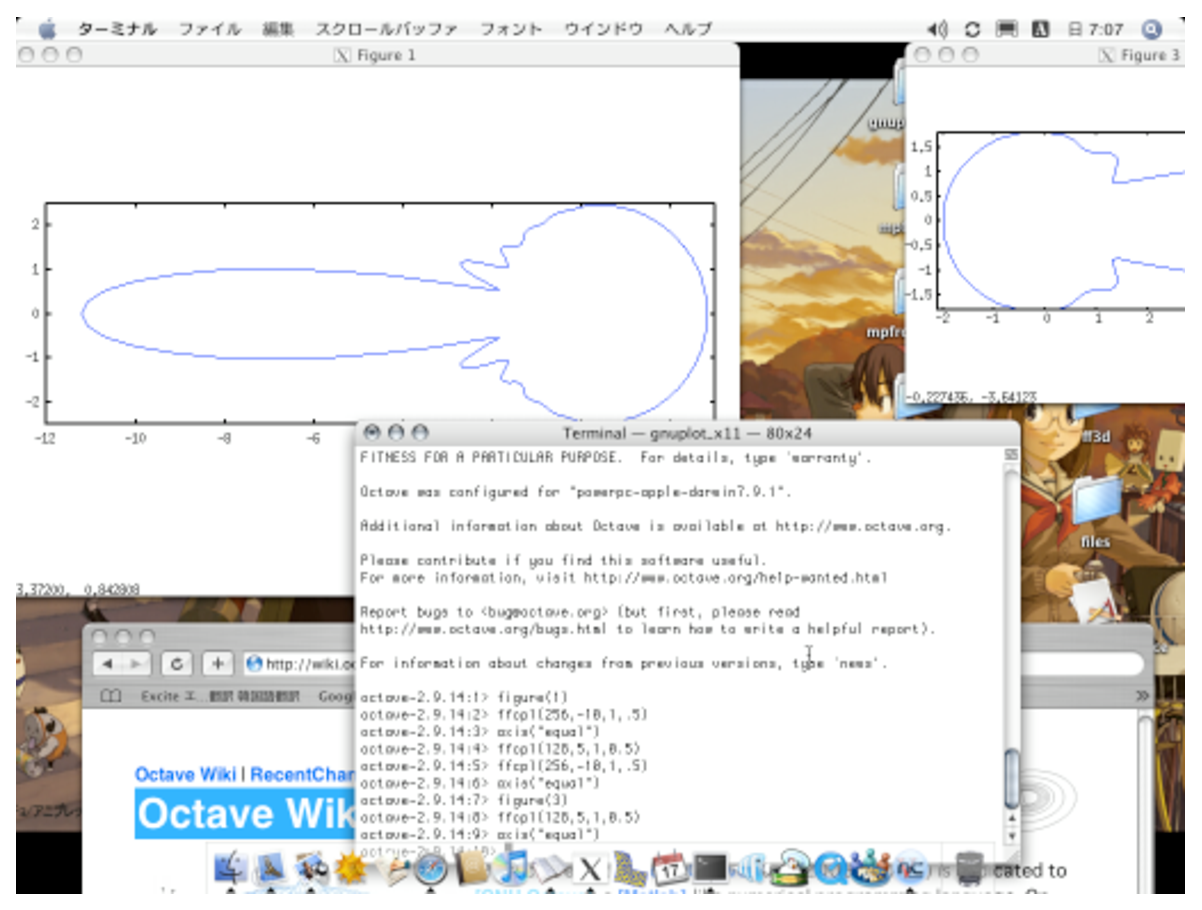
\includegraphics[scale=0.7]{./ffc1.eps}
\caption{Example of outputs for the programs}
\label{outputs}
\end{center}
\end{figure}

\begin{figure}[p]
\begin{center}
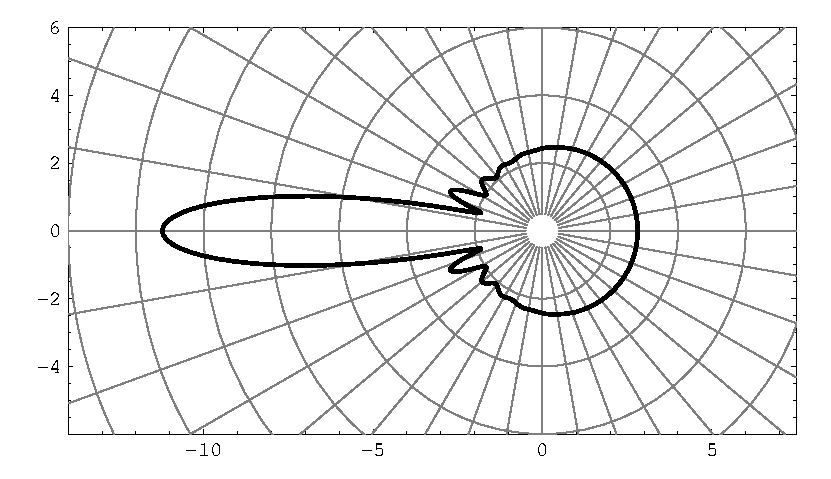
\includegraphics[scale=1]{./ffc-k10-512-05.eps}
\caption{Profile of $|P(\theta)|$ with $\kappa=ka=10$}
\label{far-field-coeff}
\end{center}
\end{figure}


\begin{figure}[p]
\begin{center}
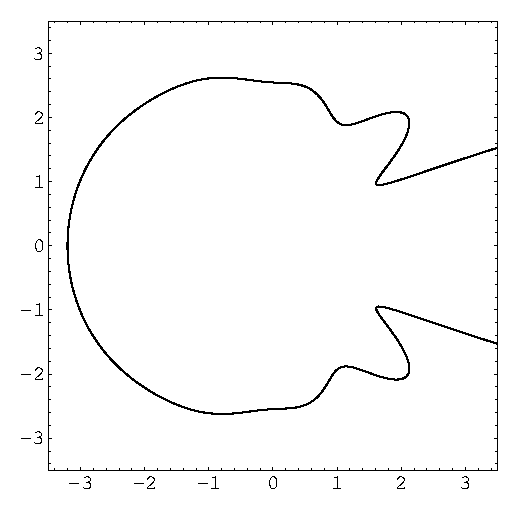
\includegraphics[scale=0.5]{./A2.eps}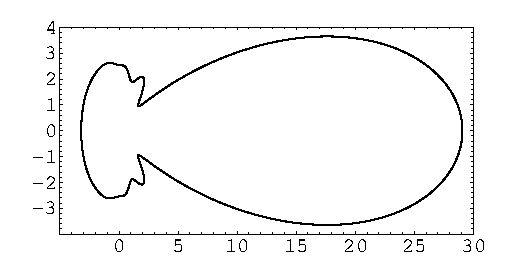
\includegraphics[scale=0.9]{./A1.eps}\\ 
{\footnotesize A: $\kappa=5$}\\
\vspace{2mm}
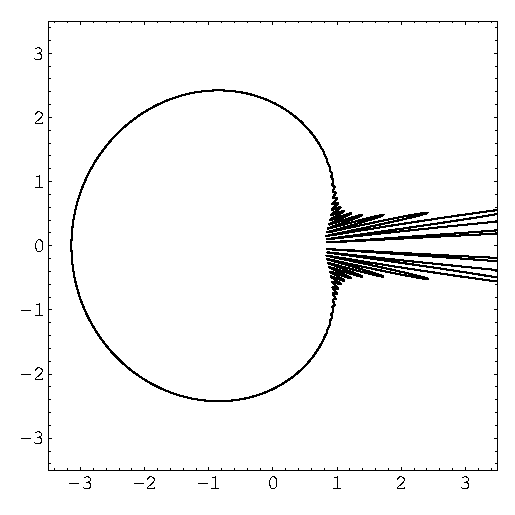
\includegraphics[scale=0.5]{./B2.eps}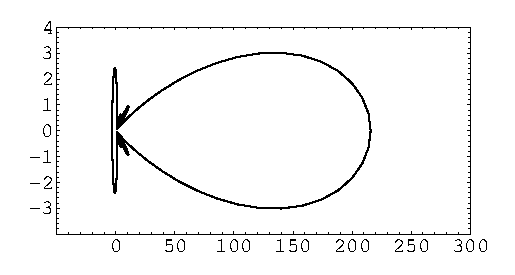
\includegraphics[scale=0.9]{./B1.eps}\\ 
{\footnotesize B: $\kappa=50$}\\
\vspace{2mm}
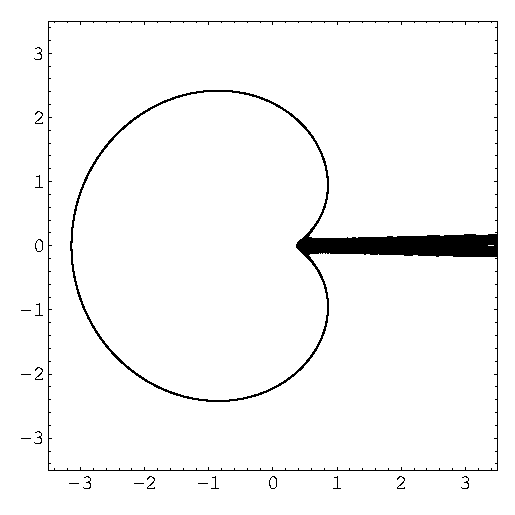
\includegraphics[scale=0.5]{./C2.eps}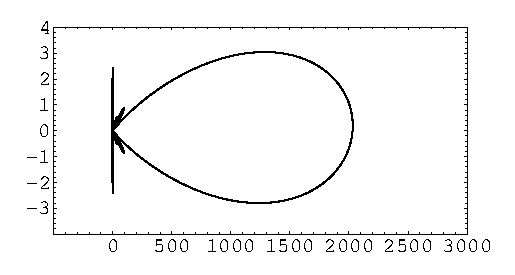
\includegraphics[scale=0.9]{./C1.eps}\\ 
{\footnotesize C: $\kappa=500$}\\
\vspace{3mm}
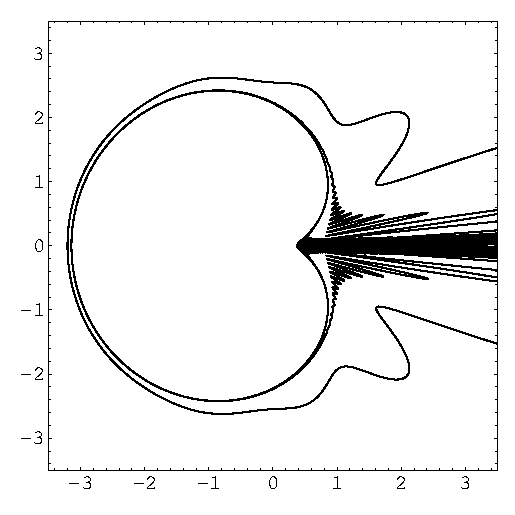
\includegraphics[scale=0.7]{./ABC.eps}\\ 
{\footnotesize D: Composite of A, B and C}\\
\caption{Scattering cross sections}
\label{fig2}
\end{center}
\end{figure}

\clearpage

\begin{thebibliography}{99}
\bibitem{Abramowitz-Stegun}
Abramowitz, M. and Stegun, I. A.,
\emph{Handbook of Mathematical Functions, with Formulas, Graphs, and Mathematical Tables}, Ninth Printing, Dover Publications, New York, 1972.

\bibitem{Bowman-Senior-Uslenghi}
Bowman, J. J., Senior, T. B. A. and Uslenghi, P. L. E.,
\emph{Electromagnetic and acoustic scattering by simple shapes}, North-Holland Publishing Company, Amsterdam, 1969.

\bibitem{eaton}
Eaton, J. W., 
{Octave - A high-level interactive language for numerical computations}, Edition 3.2.2, http://www.octave.org/, 2007.

\bibitem{ushijima-chiba 1}
Ushijima, T. and Chiba, F. ,
{A fundamental solution method for the reduced wave problem in a domain exterior to a  disc}, 
  J. Comput. Appl. Math. {\bf 152} (2002) 545--557.

\bibitem{chiba-ushijima 1}
F. Chiba, T. Ushijima and M. Ohzeki,
{A Fundamental Solution Method Applied to Reduced Wave Problems in a Domain Exterior to a Disc --- Theory, Practice and Application ---}, Kokyuroku 1566, (2007), 138--157, Research Institute for Mathematical Sciences, Kyoto University, Kyoto, (in Japanese)

\bibitem{chiba-ushijima 2}
F. Chiba and T. Ushijima, {
Computation of Scattering Amplitude for Scattering Wave by a Disc --- Approach by a Fundamental Solution Method}, Journal of Computational and Applied Mathematics, Journal of Computational and Applied Mathematics, to be appeared.
\end{thebibliography}

\end{document}
